\chapter{局域性、连续态与动量}

\lectureoverview{纠缠可以由可逆动力学产生并消除，然而当纠缠系统的一部分脱离我们的控制时，测量就变得实际上不可逆。这一区别引出一个精确的局域性检验：Bob可以在他的邻域内施加任意幺正操作，但Alice的约化密度矩阵，因而她单独可获得的每一个统计量，都保持不变。随后一个经典模拟思想实验分离出真正非经典的东西。单个自旋容易模仿，一台中心计算机也能模仿一对纠缠粒子，但彼此分离的局域机器无法在不进行非法通信、或不借助最终失败的Bell局域隐变量模型的情况下，重现所有纠缠关联。接着本讲离开自旋，转向直线上的粒子。离散求和变成积分，Kronecker delta变成Dirac delta，波函数变成无穷维空间中的矢量。乘以\(x\)给出位置；微分是反Hermite的；将其乘以\(-i\)产生Hermite的动量算符。最后的计算\([x,p]=i\hbar\)把量子对易子与经典Poisson括号重新联系起来，并指向波包、Fourier变换以及Schr\"odinger演化。}

\section{纠缠并非不可逆性}

先从一个在测量讨论中容易丢失的区别开始。假设两个自旋以乘积态到达，发生相互作用，分离，并以纠缠态离开。纠缠必须永远保持吗？不。相互作用是幺正的，所以另一个合适的相互作用可以将其消除。人们可以反射这两个自旋，使它们再次靠近，并安排一个逆演化，使这一对回到乘积态。并不存在一条定律说纠缠本身只会增加。

当这一对中的一个成员被丢弃时，情况在操作层面就改变了。如果一个电子飞入不受控制的环境，那么留在附近的伙伴仍然与某物纠缠，但缺失的自由度不再可用于逆操作。原则上，远处的电子也许可以被反射回来；实际上，它已经消失了。这就是测量\emph{对我们而言}不可逆的意义：关联已经扩散到我们无法控制的自由度中。

\begin{classroomqa}
\audiencequestion{如果两个系统变得纠缠，它们之后能变得不纠缠吗？}
\lecturerresponse{能。幺正演化是可逆的。第二次相互作用可以实现第一次的逆操作，并恢复乘积态。不可逆性出现在相关自由度被丢弃或被不受控制的环境吸收之时，而不是仅由纠缠本身产生。}
\end{classroomqa}

\begin{classroomqa}
\audiencequestion{那么为什么一次已完成的测量看起来不可逆？}
\lecturerresponse{因为被测量的系统已经与仪器、观察者、并最终与一个大环境相关联。要逆转完整状态，就需要控制所有这些记录。微观演化可以保持幺正，而该操作从观察者的约化描述来看却是不可及的。}
\end{classroomqa}

\section{Alice可用的状态}

设一个复合系统被分为Alice的自由度\(a\)和Bob的自由度\(b\)，纯态系数为
\begin{equation}
\Psi(a,b)=\braket{a,b}{\Psi}.
\end{equation}
Alice无法访问Bob的实验室。因此，她的完整局域描述一般不是一个波函数。它是约化密度矩阵
\begin{equation}
\rho_A(a',a)
=
\sum_b \Psi^*(a',b)\Psi(a,b).
\label{eq:l8-reduced-density}
\end{equation}
求和消去了Bob的标记。剩下的部分对Alice有一个bra指标和一个ket指标，并且包含Alice完全在她的邻域内进行实验所能得到的每一个概率分布。

\begin{figure}[htbp]
\centering
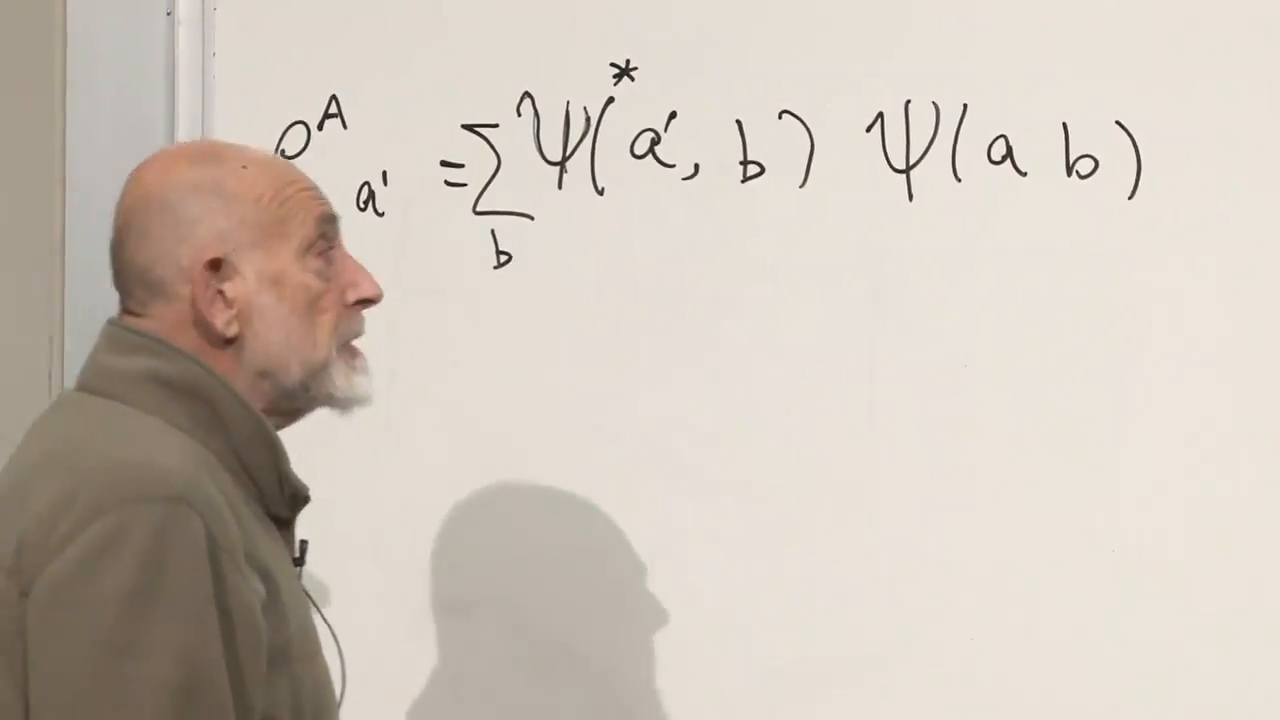
\includegraphics[width=0.88\textwidth]{lecture_08_figure_01.png}
\caption{Alice的约化密度矩阵，由联合波函数对Bob的基标记求和得到。}
\lectureframe{00:04:34}
\end{figure}

这里Alice的邻域和Bob的邻域应作广义理解。二者都可以包括仪器、磁场、技术人员，以及该观察者能够与之相互作用的任何其他自由度。局域性的主张并不是Bob不能改变他自己的系统。他可以通过许多方式这样做。主张是：当他保持远离时，他在局域所做的任何事情都不改变方程~\eqref{eq:l8-reduced-density}。

\section{Bob的局域幺正操作}

首先忽略 Alice，单独描述 Bob 的操作。如果 Bob 改变磁场或以其他方式改变他的局域哈密顿量，他的波函数系数会经历一个幺正变换，
\begin{equation}
\psi_M(b)
=
\sum_{b'}U_{bb'}\psi(b').
\label{eq:l8-bob-unitary}
\end{equation}
在复合语言中，Alice 的指标是一个旁观者：
\begin{equation}
\Psi_M(a,b)
=
\sum_{b'}U_{bb'}\Psi(a,b').
\label{eq:l8-composite-unitary}
\end{equation}
复共轭将 ket 变换转换为相应的 bra 变换，
\begin{equation}
\Psi_M^*(a',b)
=
\sum_{b''}\Psi^*(a',b'')U^\dagger_{b''b}.
\label{eq:l8-composite-bra}
\end{equation}

\begin{figure}[htbp]
\centering
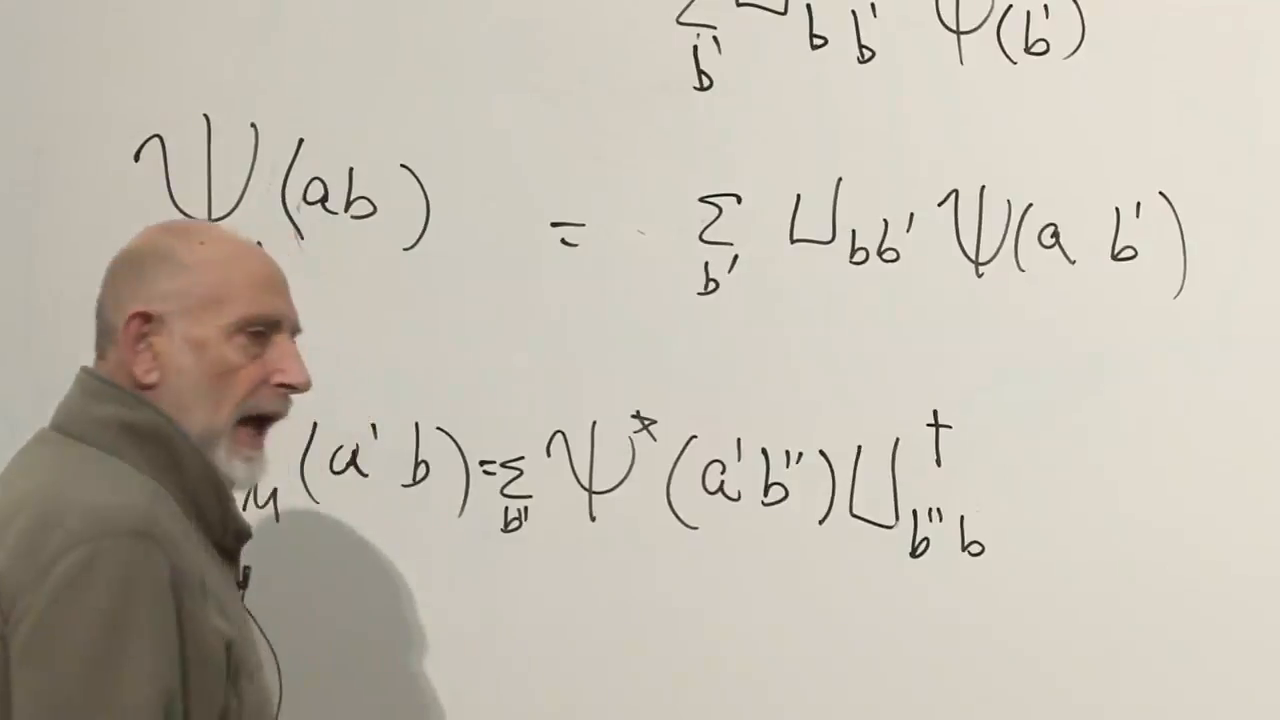
\includegraphics[width=0.88\textwidth]{lecture_08_figure_02.png}
\caption{一个幺正算符作用在 Bob 的 ket 指标上，而厄米共轭矩阵作用在相应的 bra 指标上。}
\lectureframe{00:12:54}
\end{figure}

现在重新计算 Alice 的密度矩阵：
\begin{align}
\rho_{A,M}(a',a)
&=
\sum_b\Psi_M^*(a',b)\Psi_M(a,b) \notag\\
&=
\sum_{b,b',b''}
\Psi^*(a',b'')
U^\dagger_{b''b}U_{bb'}
\Psi(a,b') \notag\\
&=
\sum_{b',b''}
\Psi^*(a',b'')
(U^\dagger U)_{b''b'}
\Psi(a,b') \notag\\
&=
\sum_{b',b''}
\Psi^*(a',b'')\delta_{b''b'}\Psi(a,b') \notag\\
&=
\sum_{b'}\Psi^*(a',b')\Psi(a,b') \notag\\
&=
\rho_A(a',a).
\label{eq:l8-locality-proof}
\end{align}

\begin{figure}[htbp]
\centering
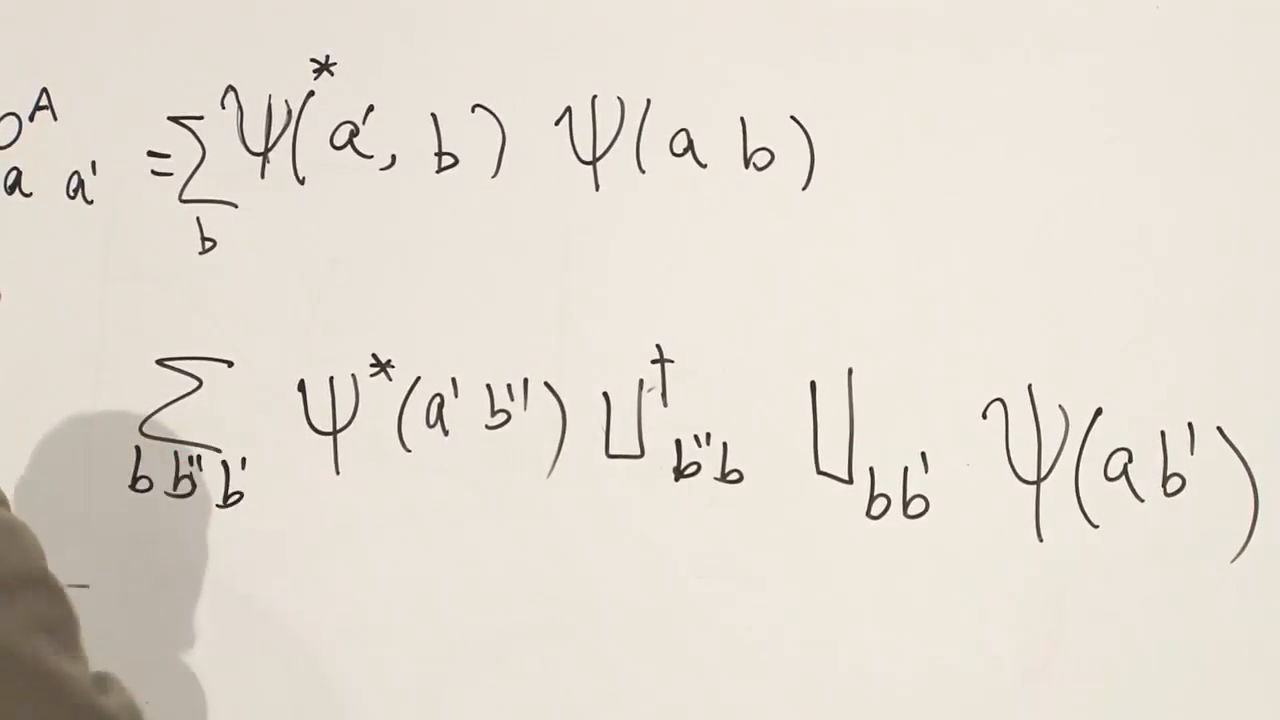
\includegraphics[width=0.88\textwidth]{lecture_08_figure_03.png}
\caption{黑板上的定域性计算：\(U^\dagger U\) 在 Alice 的约化态内部收缩为单位矩阵。}
\lectureframe{00:14:27}
\end{figure}

整个证明就是收缩
\begin{equation}
\sum_bU^\dagger_{b''b}U_{bb'}
=(U^\dagger U)_{b''b'}
=\delta_{b''b'}.
\label{eq:l8-unitarity-contraction}
\end{equation}
没有使用任何因子化假设。方程~\eqref{eq:l8-locality-proof} 无论联合态是乘积态还是最大纠缠态都成立。因此每一个仅涉及 Alice 的期望值，
\begin{equation}
\expect{L_A}
=
\operatorname{Tr}_A(\rho_A L_A),
\end{equation}
在 Bob 的局域幺正变换下不变。

\begin{classroomqa}
\audiencequestion{如果 Bob 对他的自旋做了些什么，为什么这还不算已经违反幺正性？}
\lecturerresponse{做了些什么并不意味着施加一个非幺正映射。Bob 可以旋转磁铁、改变局域哈密顿量，或者让他的自旋进动。这些都是普通的幺正演化。它们改变他自己的态和他自己的结果概率，但上面的计算表明它们不改变 Alice 的约化态。}
\end{classroomqa}

\begin{classroomqa}
\audiencequestion{那么量子力学是否因此服从定域性？}
\lecturerresponse{它服从这里使用的操作定域性：Bob 仅在他的邻域内行动，不能影响 Alice 可进行的测量的统计。纠缠的联合关联仍然是非经典的，但它们不提供可控的信号。}
\end{classroomqa}

\subsection{为什么幺正性重要}

幺正性并非装饰性的。它提供了方程~\eqref{eq:l8-unitarity-contraction} 中的单位矩阵。用先前的语言来说，幺正性表达了区别的守恒：两个可区分的态矢量在可逆演化下仍然可区分。如果 Bob 拥有哪怕稍微非幺正的确定性演化，\(U^\dagger U\) 就不会是单位矩阵。Alice 的约化密度矩阵那时就可能立即改变，从而给 Bob 一种超光速发信号的手段。

这种紧密联系是量子力学难以零敲碎打地修改的原因之一。改变演化定律，表面上遥远的原理也可能随之失效。定域性、概率守恒和可逆态演化是同一个结构的组成部分。

\begin{classroomqa}
\audiencequestion{非幺正操作如何允许超光速信号？}
\lecturerresponse{Bob 会选择是否施加它。如果该映射改变了 \(\rho_A\)，Alice 就可以通过对系综重复局域测量来区分这两种选择。这种改变会在没有信号从 Bob 传播过来的情况下发生，而这正是幺正抵消所阻止的。}
\end{classroomqa}

\section{坍缩改变的是条件，而非远处的边缘分布}

分束器例子使这种不安变得生动。一个单光子被置于两条路径的叠加态中，一条朝向 Alice，一条朝向 Bob。如果 Alice 的探测器咔嗒响，条件态就给 Bob 路径上后来的咔嗒声赋予零振幅。人们很容易说 Alice 瞬时改变了 Bob 的光子。

Bob 在没有 Alice 记录的情况下所能观察到的是不同的。在收到任何消息之前，他必须对 Alice 的可能结果取平均。那个无条件平均由他的约化密度矩阵描述，而它不会改变。Alice 的咔嗒声改变的是：一旦她的结果已知，哪个条件子系综描述一次运行；它不改变 Bob 的局域边缘分布。
\begin{equation}
\rho_B
\qquad\text{and}\qquad
\rho_{B\mid A=\text{click}}
\end{equation}
之间的区别，就是无信号与有用关联之间的区别。

\begin{classroomqa}
\audiencequestion{当一个探测器咔嗒响时，另一条臂上的波函数难道不是瞬时坍缩为零吗？}
\lecturerresponse{以那次咔嗒声为条件的状态会改变，但远处的观察者在普通消息到达之前并不拥有这个条件。Bob 的无条件密度矩阵以及他所有平均局域统计都保持不变。坍缩不能被用作电报。}
\end{classroomqa}

\begin{classroomqa}
\audiencequestion{这种混淆是否部分地是状态与关于状态的信息之间的混淆？}
\lecturerresponse{这种说法有启发性，但仍然过于松散。具体的区分在于联合态、约化态以及以所报告的结果为条件的状态之间。把这三个数学对象分开来对待，比试图仅凭“信息”一词来解决问题更为稳妥。}
\end{classroomqa}

然而，爱因斯坦--波多尔斯基--罗森式的不适依然存在。单态可以让我们对\emph{整体}拥有最大限度的知识，而两个组成部分却都没有纯的局域态。这种对经典预期的颠倒---即知道整体却不给部分指定确定的纯态---并不是一种信号传递效应，但它确实很奇特。为了更尖锐地揭示这种奇特性，把量子力学变成一个编程问题。

\section{一个自旋的经典模拟器}

在计算机屏幕上画出一个自旋装置。用户可以调整它的方向，按下测量按钮\(M\)，并读取\(+1\)或\(-1\)。在经典计算机内部存储两个复振幅，
\begin{equation}
\alpha_u,\qquad \alpha_d,
\qquad
|\alpha_u|^2+|\alpha_d|^2=1.
\label{eq:l8-one-spin-amplitudes}
\end{equation}
在两次测量之间，计算机对相应的Schr\"odinger方程进行积分。模拟的磁场可以使振幅像真实自旋态那样精确进动。

\begin{figure}[htbp]
\centering
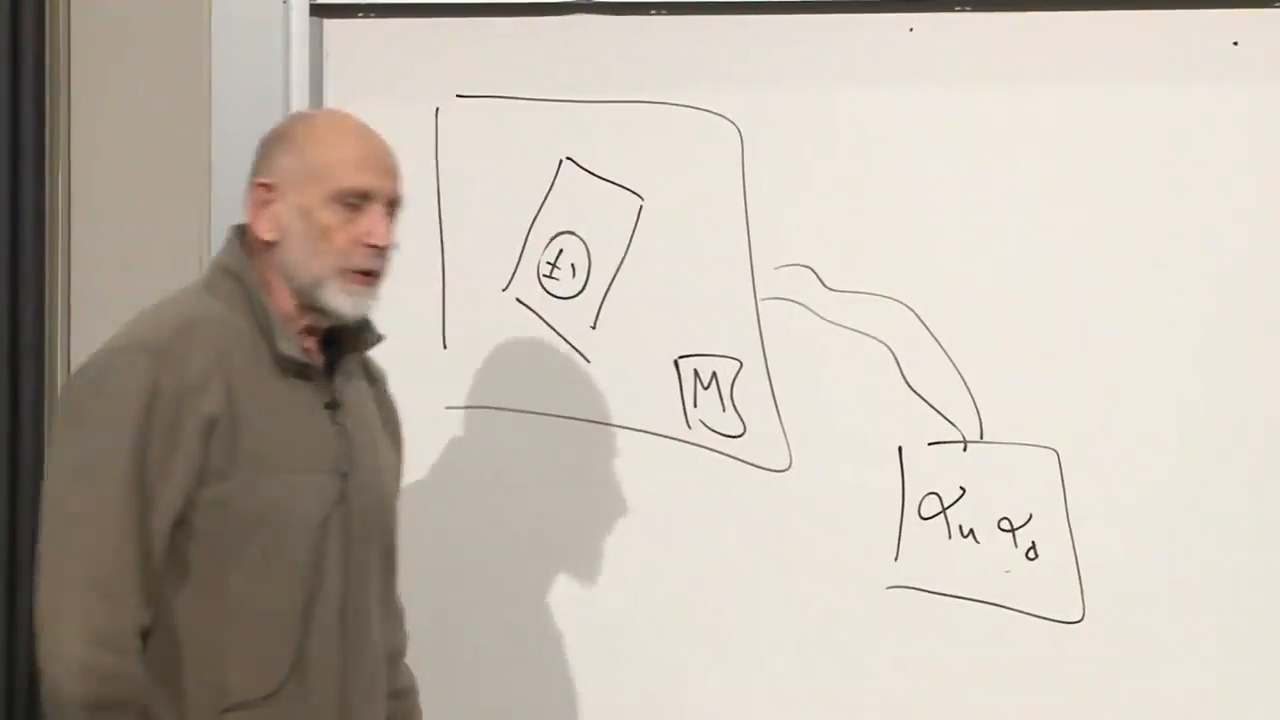
\includegraphics[width=0.88\textwidth]{lecture_08_figure_04.png}
\caption{单自旋模拟器：一个可调整方向的装置和测量按钮，连接着一台存储两个振幅的计算机。}
\lectureframe{00:27:47}
\end{figure}

当用户按下\(M\)时，一个伪随机数发生器按照玻恩概率选择一个结果
\begin{equation}
P(+1)=|\alpha_u|^2,
\qquad
P(-1)=|\alpha_d|^2.
\label{eq:l8-one-spin-born}
\end{equation}
计算机显示所选的符号，然后执行状态更新。在\(+1\)之后，
\begin{equation}
(\alpha_u,\alpha_d)\longrightarrow(1,0),
\end{equation}
而在\(-1\)之后，
\begin{equation}
(\alpha_u,\alpha_d)\longrightarrow(0,1).
\end{equation}
然后它从测量后的状态继续幺正演化。如果用户在按下\(M\)之前旋转装置，计算机就改变基，并计算适合新轴的概率。

硬件并不需要任何特定的量子特性。一个确定性的伪随机算法就足以产生对用户来说看似随机的序列。对于单个自旋，这种经典模仿在操作上可以与实验室实验无法区分。

\begin{classroomqa}
\audiencequestion{测量按钮的目的是什么？在按下它之前，经过的时间重要吗？}
\lecturerresponse{按钮标志着模拟器对玻恩分布进行采样并更新所存储振幅的时刻。在等待期间，振幅在哈密顿量下演化。如果哈密顿量为零，则什么都不随时间改变；如果有磁场，模拟的自旋在测量之前会进动。}
\end{classroomqa}

\begin{classroomqa}
\audiencequestion{谁决定何时按下按钮，或者把装置朝哪个方向调整？}
\lecturerresponse{在这个模型中，实验者提供这些设置。模拟器持续跟踪状态，然后在按下按钮时使用所选的轴和测量时间。后面的讨论将回到这样一个假设：设置可以独立于所制备的粒子对而被选择。}
\end{classroomqa}

\section{两个自旋：局域模拟在哪里失败}

处于乘积态的两个自旋仍然很容易。给爱丽丝一台存储振幅\(\alpha_u,\alpha_d\)的计算机，给鲍勃另一台存储\(\beta_u,\beta_d\)的计算机。每台机器演化并测量自己的自旋。不需要通信，因为联合系数可以分解：
\begin{equation}
\Psi(a,b)=\alpha_a\beta_b.
\end{equation}

任意的双自旋态需要四个系数，
\begin{equation}
\alpha_{uu},\qquad
\alpha_{ud},\qquad
\alpha_{du},\qquad
\alpha_{dd},
\qquad
\sum_{a,b}|\alpha_{ab}|^2=1.
\label{eq:l8-four-amplitudes}
\end{equation}
一台单一的中央计算机可以存储这些数，并用四维Schr\"odinger方程演化它们。当任一观察者测量时，中央机器对正确的边缘概率进行采样，丢弃不相容的分量，对存活的分量重新归一化，并从条件态继续。

\begin{figure}[htbp]
\centering
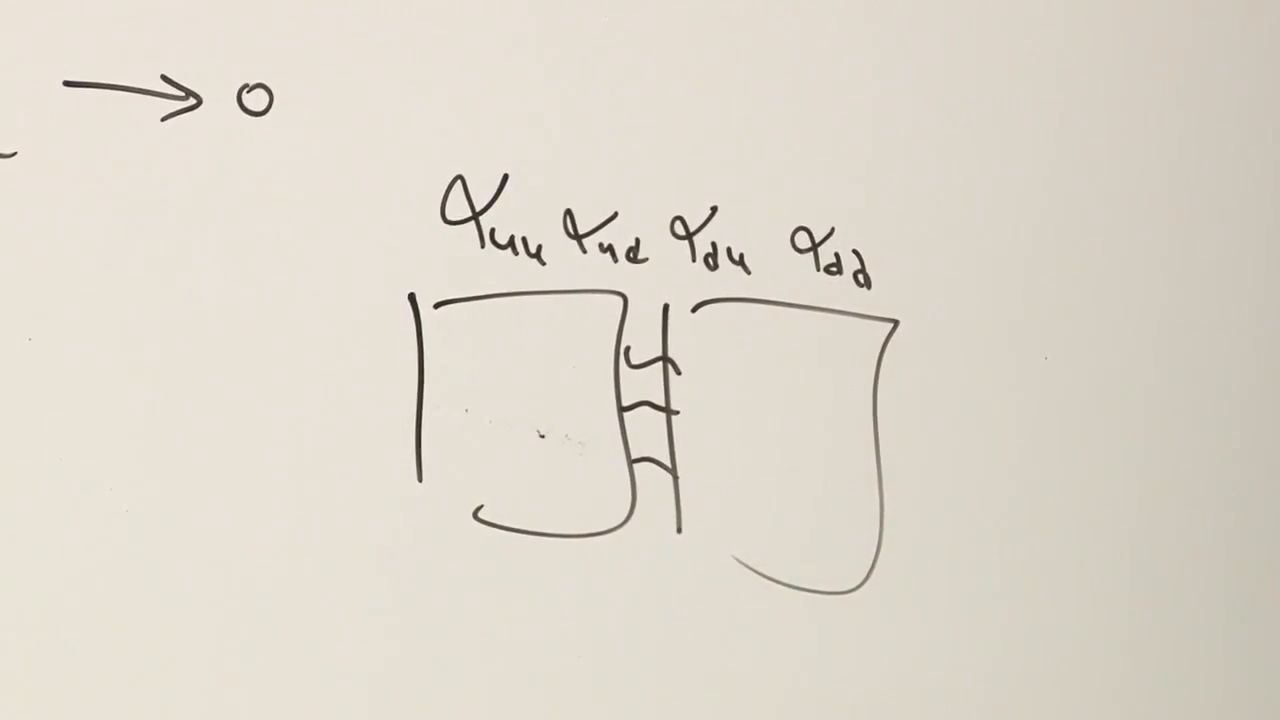
\includegraphics[width=0.88\textwidth]{lecture_08_figure_05.png}
\caption{一台中央模拟器存储任意双自旋态的四个振幅，并保持与两个测量站相连。}
\lectureframe{00:37:47}
\end{figure}

只要中央处理器保持与两侧相连，这种构造就能完美地模拟纠缠。当人们把四个振幅复制到两台机器中，将它们分开，切断连线，并让每台机器使用自己的随机发生器时，麻烦就开始了。对于单态，
\begin{equation}
\ket{\Psi^-}
=
\frac{1}{\sqrt2}
\left(
\ket{u}_A\ket{d}_B-\ket{d}_A\ket{u}_B
\right),
\label{eq:l8-singlet}
\end{equation}
同轴测量必须相反。独立的随机选择反而可能产生\(++\)或\(--\)，因此即使两台机器一开始都拥有联合系数的副本，关联也丢失了。

\begin{classroomqa}
\audiencequestion{在分离之前，两台机器能否共享同一个随机数源？}
\lecturerresponse{共享随机性可以为某一个固定测量轴强制实现预先规定的关联。更深刻的贝尔问题要求存在一个局域方案，能够对每一对独立选定的轴都再现量子关联。预载的共享变量也被包含在贝尔局域模型之中，而没有任何这样的模型能再现完整的量子关联函数。}
\end{classroomqa}

\begin{classroomqa}
\audiencequestion{这四个振幅是独立的吗？}
\lecturerresponse{它们是一个归一化联合态的四个坐标，而不是四个独立的局域态。在纠缠态中，它们不能写成\(\alpha_a\beta_b\)。当一个局域结果被选定后，存留下来的联合系数必须被相干地更新；两个互不连接的副本并不会自动执行相匹配的更新。}
\end{classroomqa}

\subsection{隐藏导线意味着什么}

一个连接到两个站点的中心随机发生器可以协调输出。在普通的经典模拟器中，那些导线同时也会是通信信道。Bob可以有意向Alice发送一个比特，而如果该链路是瞬时的，这台机器就会违反定域性。

量子系统并不给予Bob那种自由。他所能进行的局域变换是幺正的，而约化密度矩阵的证明已经表明，任何这样的变换都不会改变Alice的边缘统计。因此，模拟器的导线表明的是普通经典记账方式具有错误的结构，而不是自然界中存在可获取的超光速缆线。

\begin{classroomqa}
\audiencequestion{经典模拟器所需的那些导线是否代表物理上的非定域性？}
\lecturerresponse{它们代表的是一个朴素的经典模型所需的额外协调。如果它们是普通可用的导线，它们就会允许信号传递，也就不能模拟量子实验。更稳妥的结论是：局域经典模拟与量子力学具有不同的逻辑结构，而不是发现了隐藏的通信导线。}
\end{classroomqa}

\begin{classroomqa}
\audiencequestion{如果Alice和Bob各自收到一个随机比特，但这些比特完全关联，这有什么奇怪之处？}
\lecturerresponse{一个预先安排好的关联本身并不奇怪；相同的信封或共享的随机种子都能产生它。非经典内容出现在Alice和Bob在互不相容的设置中独立选择，而由此产生的关联违反贝尔不等式，同时每个局域结果仍保持随机之时。}
\end{classroomqa}

这个思想实验还包含一个值得阐明的预设：测量设置被当作独立选择。Alice和Bob决定何时按下按钮以及如何取向他们的装置，而这些选择并不被源变量暗中固定。一旦观察者及其决策机制被包含在一个封闭物理系统之内，自由选择的哲学语言就变得微妙起来。操作性的贝尔检验把所需条件表述为测量独立性，并安排类空间隔的、外部生成的设置。本讲对形而上学问题保持开放，同时保留实验预设。

\begin{classroomqa}
\audiencequestion{把Alice和Bob放进物理系统之内是否造成了一个漏洞？}
\lecturerresponse{它揭示了一个假设：设置不能事先与制备该对粒子的隐变量相关联。人们可以争论自由意志，但可检验的陈述是测量独立性。放弃它在逻辑上是可能的，不过那只是改变了说明负担，而不是提供一种普通的局域模拟。}
\end{classroomqa}

\section{从自旋到直线上的一个粒子}

自旋已经把讨论从有限维矢量带到了纠缠和定域性。现在扩大希尔伯特空间。考虑一个在无限直线上运动的粒子。位置本征态记为
\begin{equation}
\ket{x},
\end{equation}
它意味着粒子具有确定的位置\(x\)。这些右矢构成一个连续标记的基。一般态是它们的叠加，其位置空间波函数为
\begin{equation}
\psi(x)=\braket{x}{\Psi}.
\label{eq:l8-position-wavefunction}
\end{equation}

\begin{figure}[htbp]
\centering
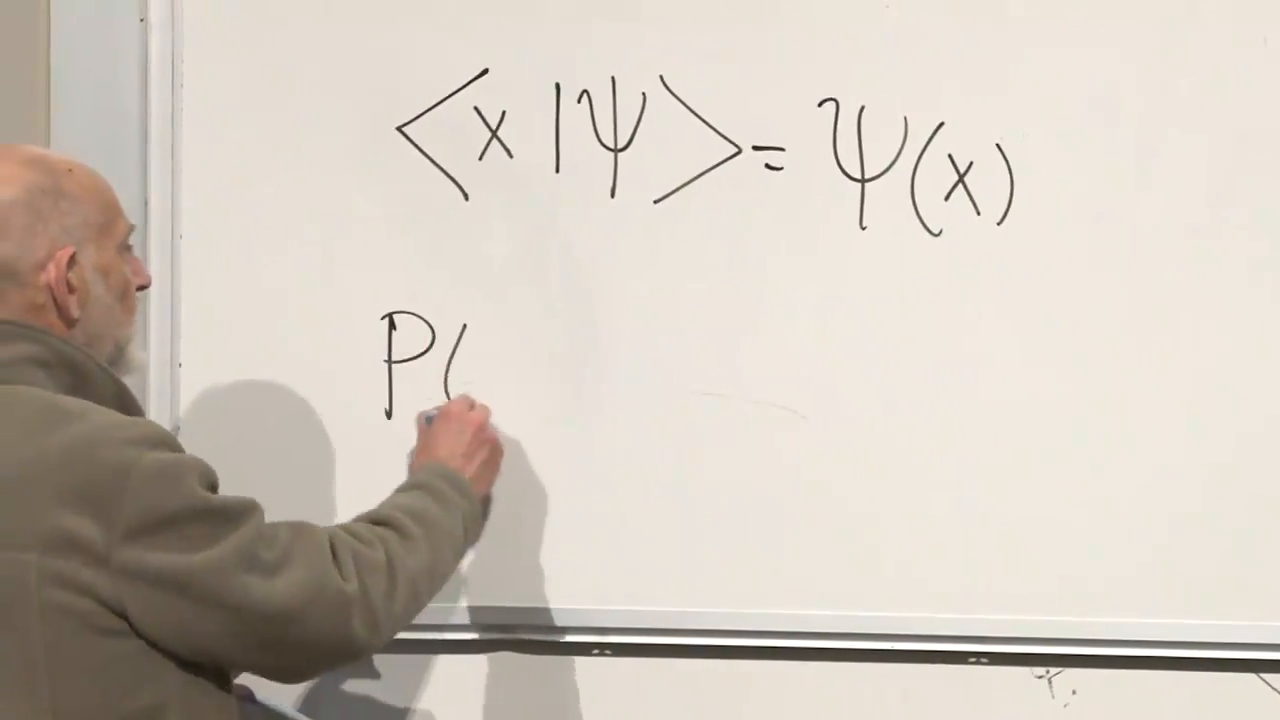
\includegraphics[width=0.88\textwidth]{lecture_08_figure_06.png}
\caption{位置空间波函数是抽象态在基右矢\(\ket{x}\)上的投影。}
\lectureframe{00:56:51}
\end{figure}

这里把位置用作一个完备的基标记。这并不意味着一个经典态可以仅由位置来指定，也不意味着粒子同时具有确定的位置和动量。它意味着每一个量子态矢量都可以在位置基中展开。动量将作为作用于那些位置空间系数上的算符出现。

玻恩规则现在给出概率\emph{密度}，
\begin{equation}
\rho(x)=|\psi(x)|^2.
\label{eq:l8-probability-density}
\end{equation}
对于连续变量，一个确切点的概率通常为零。在某一区间内找到粒子的概率为
\begin{equation}
P(x_1<x<x_2)
=
\int_{x_1}^{x_2}|\psi(x)|^2\,dx,
\end{equation}
而归一化要求
\begin{equation}
\int_{-\infty}^{\infty}|\psi(x)|^2\,dx=1.
\label{eq:l8-continuous-normalization}
\end{equation}

\begin{classroomqa}
\audiencequestion{当经典粒子同时需要位置和动量时，仅凭位置怎么能构成完备基？}
\lecturerresponse{这里的完备性涉及量子矢量的表示。所有\(x\)对应的系数\(\psi(x)\)确定了态，而动量信息编码在它们的相位和空间变化中。位置和动量是不同的基，稍后通过傅里叶变换相联系；它们不是同时成立的经典标签。}
\end{classroomqa}

\begin{classroomqa}
\audiencequestion{\(|\psi(x)|^2\)是在确切点\(x\)找到粒子的概率吗？}
\lecturerresponse{它是一个密度。乘以一个小区间\(dx\)给出该区间内的近似概率，而积分给出有限区域的精确概率。即使赋予一个孤立点的概率为零，密度也可以非零。}
\end{classroomqa}

\section{连续正交归一性与{\proseunicodefont δ}函数}

对于离散正交归一基，
\begin{equation}
\braket{a}{a'}=\delta_{aa'}.
\end{equation}
对于连续基，其类似式为
\begin{equation}
\braket{x}{x'}=\delta(x-x'),
\label{eq:l8-delta-normalization}
\end{equation}
其中狄拉克{\proseunicodefont δ}在\(x\neq x'\)时为零，且具有单位面积：
\begin{equation}
\int_{-\infty}^{\infty}\delta(x-x')\,dx'=1.
\end{equation}
可以把它想象为一个宽度为\(\epsilon\)、高度为\(1/\epsilon\)、面积固定的窄尖峰，然后取极限\(\epsilon\to0\)。

\begin{figure}[htbp]
\centering
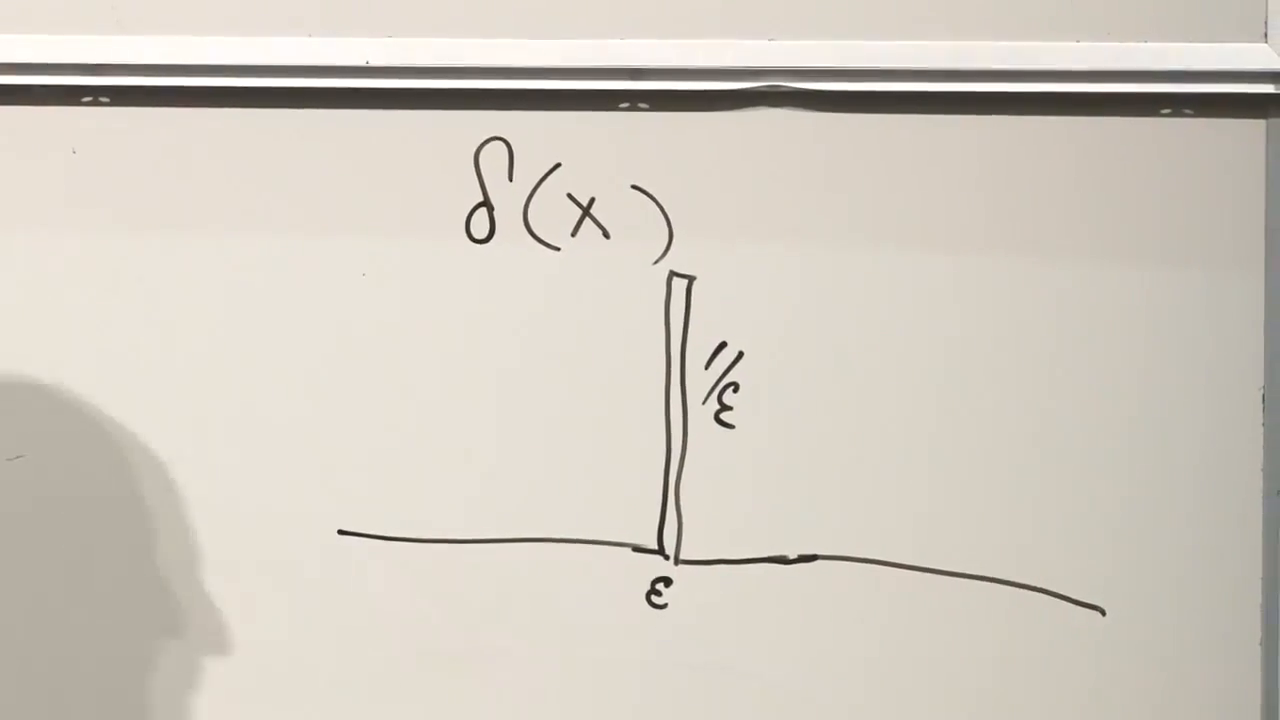
\includegraphics[width=0.88\textwidth]{lecture_08_figure_07.png}
\caption{黑板上对狄拉克{\proseunicodefont δ}的窄尖峰表示：宽度\(\epsilon\)、高度\(1/\epsilon\)、单位面积。}
\lectureframe{01:01:57}
\end{figure}

这种记号是分布意义下的简写。位置本征右矢不是普通平方可积希尔伯特空间中的可归一化矢量；它是一个广义矢量，其{\proseunicodefont δ}归一化只有在积分下才有意义。核心工作规则是
\begin{equation}
\int_{-\infty}^{\infty}
\delta(x-x')f(x')\,dx'
=f(x).
\label{eq:l8-delta-sampling}
\end{equation}
{\proseunicodefont δ}挑选出其自变量为零时的值。

现在写出连续展开
\begin{equation}
\ket{\Psi}
=
\int_{-\infty}^{\infty}
\psi(x')\ket{x'}\,dx'.
\label{eq:l8-continuous-expansion}
\end{equation}
用\(\bra{x}\)作用给出
\begin{align}
\braket{x}{\Psi}
&=
\int dx'\,\psi(x')\braket{x}{x'} \notag\\
&=
\int dx'\,\psi(x')\delta(x-x') \notag\\
&=
\psi(x).
\label{eq:l8-expansion-consistency}
\end{align}
因此，展开中的系数与投影\(\braket{x}{\Psi}\)是同一个函数，正如离散基中的情形一样。

\begin{figure}[htbp]
\centering
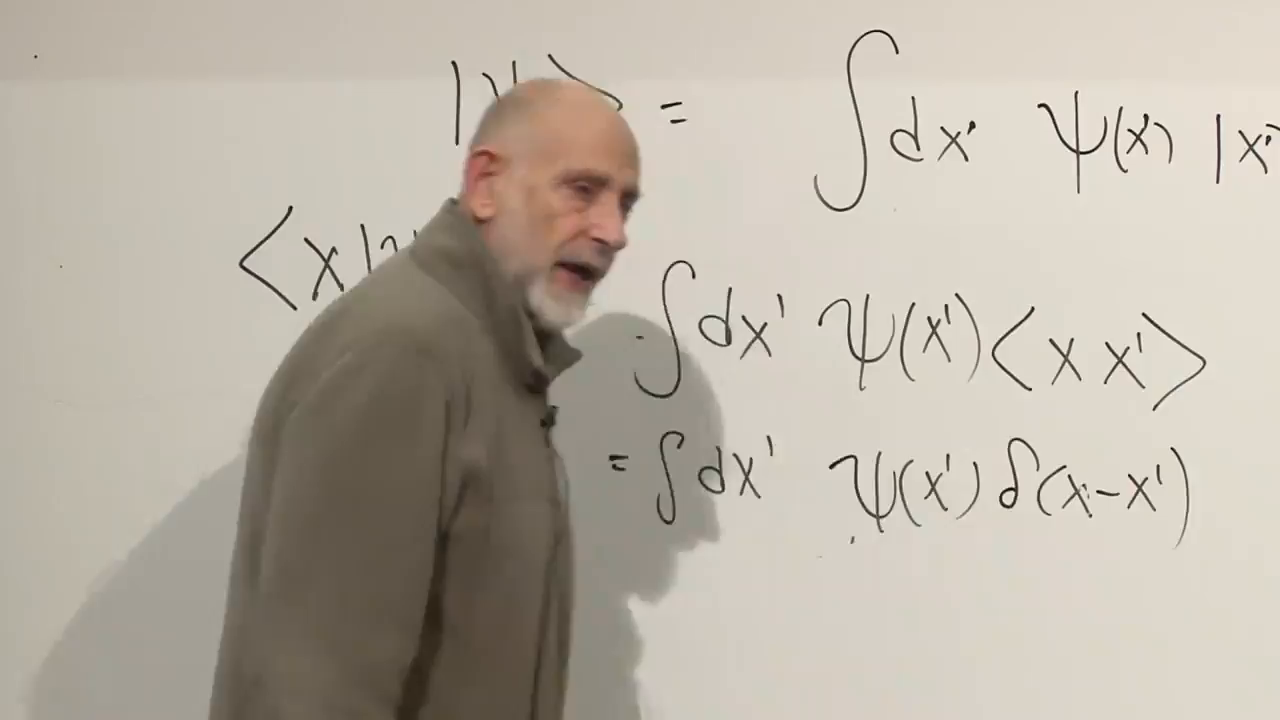
\includegraphics[width=0.88\textwidth]{lecture_08_figure_08.png}
\caption{连续态展开及其使用\(\braket{x}{x'}=\delta(x-x')\)的一致性检验。}
\lectureframe{01:07:00}
\end{figure}

\begin{classroomqa}
\audiencequestion{\(\psi(x')\)是否扮演与有限维矢量中的振幅相同的角色？}
\lecturerresponse{是的。基标签\(a'\)变为连续标签\(x'\)，求和变为积分，系数\(\psi(a')\)变为函数\(\psi(x')\)。底层的矢量空间陈述保持不变。}
\end{classroomqa}

\begin{classroomqa}
\audiencequestion{狄拉克{\proseunicodefont δ}真的是一个在某一点取无限值的函数吗？}
\lecturerresponse{这种图像有用，但并非字面意义。严格地说，{\proseunicodefont δ}是由其在积分下的作用定义的分布，即方程~\eqref{eq:l8-delta-sampling}。窄的单位面积尖峰是一列普通函数，它们趋近于同一采样规则。}
\end{classroomqa}

\section{函数作为矢量}

为了看出内积，首先回忆离散计算：
\begin{align}
\braket{\psi}{\phi}
&=
\sum_{a',a}
\psi^*(a')\braket{a'}{a}\phi(a) \notag\\
&=
\sum_a\psi^*(a)\phi(a).
\label{eq:l8-discrete-inner-product}
\end{align}
复共轭的系数属于左矢，而正交归一性使双重求和坍缩。

\begin{figure}[htbp]
\centering
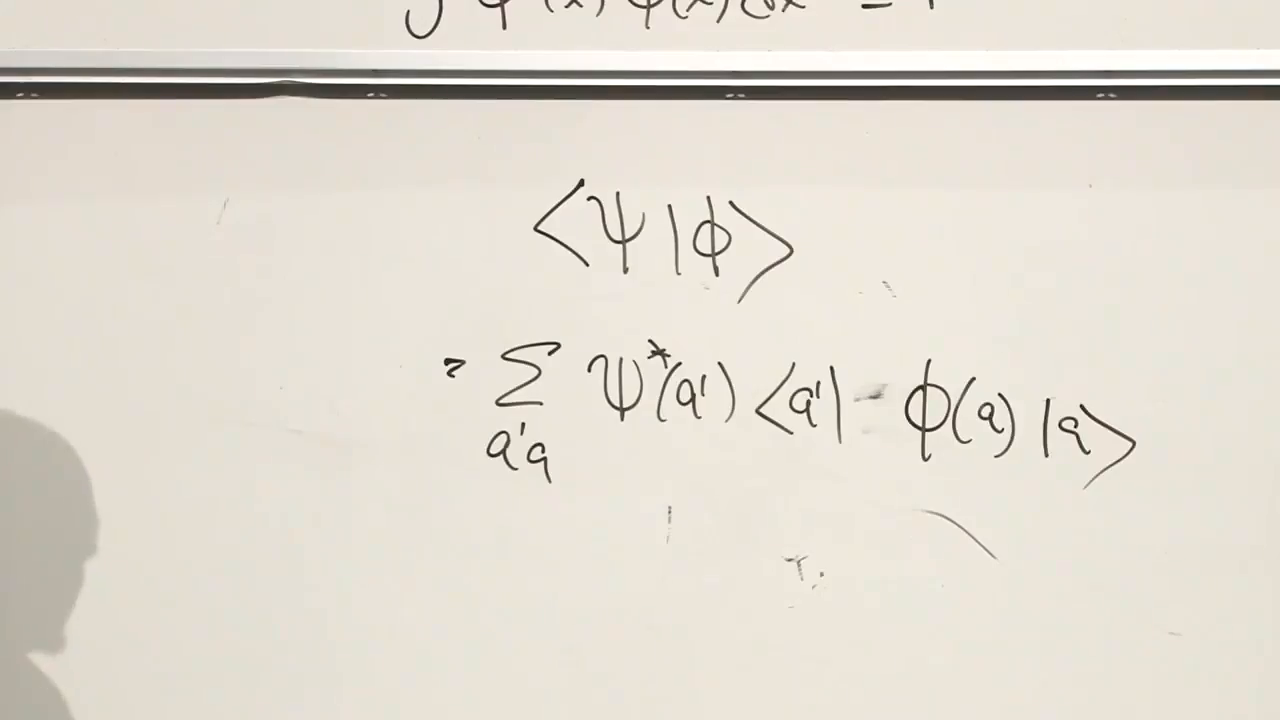
\includegraphics[width=0.88\textwidth]{lecture_08_figure_09.png}
\caption{在求和被积分替换之前，按基展开的离散内积。}
\lectureframe{01:11:11}
\end{figure}

把基标签替换为位置，把求和替换为积分：
\begin{equation}
\braket{\psi}{\phi}
=
\int_{-\infty}^{\infty}\psi^*(x)\phi(x)\,dx.
\label{eq:l8-continuous-inner-product}
\end{equation}
交换两个矢量会使结果取复共轭，
\begin{equation}
\braket{\phi}{\psi}
=
\braket{\psi}{\phi}^*,
\end{equation}
而范数为
\begin{equation}
\|\psi\|^2=\braket{\psi}{\psi}
=\int |\psi(x)|^2\,dx.
\end{equation}

因此函数就是矢量：它们可以相加、乘以复标量、归一化，并通过内积配对。无限直线上的物理波函数是平方可积的，因此在无穷远处无界增长的函数被排除。广义基函数\(\delta(x-x_0)\)恰好位于该希尔伯特空间之外，但作为分布意义下的基矢量仍然不可或缺。

\begin{classroomqa}
\audiencequestion{未标明的积分限应当是\(-\infty\)和\(+\infty\)吗？}
\lecturerresponse{是的，对于无限直线而言。这些积分限也解释了为什么可归一化波函数必须衰减得足够快：否则总概率积分将不存在。}
\end{classroomqa}

\begin{classroomqa}
\audiencequestion{黑板上的一个表达式中少了一条竖线。这会改变它的含义吗？}
\lecturerresponse{那只是一个记号上的疏漏。基矢的重叠是 \(\braket{a'}{a}\)，左边是左矢，右边是右矢。补上竖线后就能清楚地看出，这个表达式是一个内积，而不是一个含糊的行或列。}
\end{classroomqa}

\begin{classroomqa}
\audiencequestion{在大多数时候，几乎一切事物都与环境纠缠在一起吗？}
\lecturerresponse{在现实的宏观条件下，是的。系统不断受到光子、空气分子以及其他自由度的撞击，把相位信息扩散到环境中。这种环境纠缠是退相干的核心，也是宏观备选方案之间的干涉难以被观测到的原因。}
\end{classroomqa}

\begin{classroomqa}
\audiencequestion{分布论的数学理论改变了物理学，还是仅仅让 delta 函数变得体面了？}
\lecturerresponse{它最直接的作用是使物理学家已经在使用的操作变得严格。它为广义函数提供了精确的语言，并减少了与数学家之间的争论，尽管它本身并未解决量子场论中所有的分布论困难。}
\end{classroomqa}

\section{波函数上的线性算符}

线性算符把一个函数映射为另一个函数，同时保持叠加性：
\begin{equation}
L(c_1\psi+c_2\phi)
=
c_1L\psi+c_2L\phi.
\end{equation}
可观测量必须由厄米算符表示。在目前的记号下，条件是
\begin{equation}
\braket{\phi}{L\psi}
=
\braket{L\phi}{\psi},
\label{eq:l8-hermitian-condition}
\end{equation}
或者等价地
\begin{equation}
\braket{\phi}{L\psi}
=
\braket{\psi}{L\phi}^*.
\end{equation}
对于无界算符，这一陈述包含定义域和边界条件；下面的积分假定波函数使边界项为零。

\subsection{位置即乘法}

最简单的算符是用坐标乘以波函数：
\begin{equation}
(x\psi)(x)=x\psi(x).
\label{eq:l8-position-operator}
\end{equation}
它是线性的，并且
\begin{align}
\braket{\phi}{x\psi}
&=
\int dx\,\phi^*(x)x\psi(x), \notag\\
\braket{x\phi}{\psi}
&=
\int dx\,[x\phi(x)]^*\psi(x) \notag\\
&=
\int dx\,\phi^*(x)x\psi(x),
\end{align}
因为 \(x\) 是实数。因此，乘以 \(x\) 是厄米的，并表示位置可观测量。

\begin{figure}[htbp]
\centering
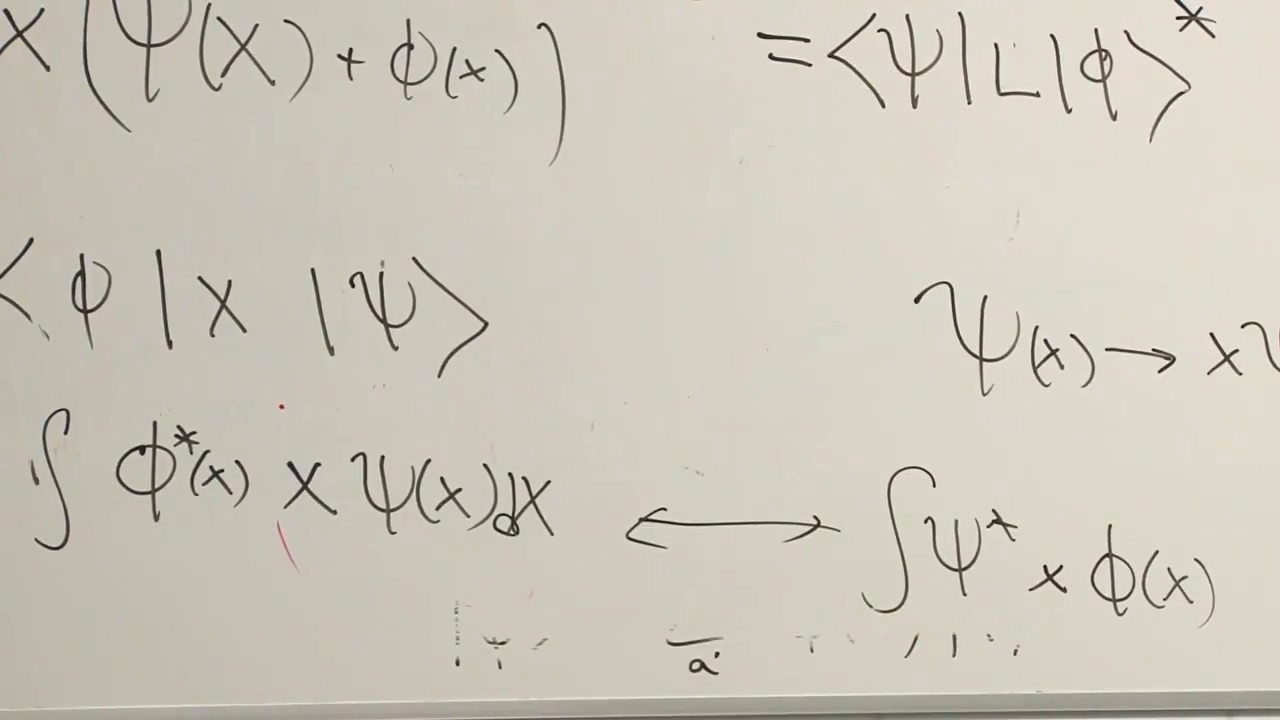
\includegraphics[width=0.88\textwidth]{lecture_08_figure_10.png}
\caption{位置算符的厄米性检验，该算符可视为用实变量 \(x\) 乘以波函数。}
\lectureframe{01:26:47}
\end{figure}

\begin{classroomqa}
\audiencequestion{在 \(x\psi(x)\) 中，\(x\) 是一个算符，还是仅仅是一个实数？}
\lecturerresponse{在每一点上，它是实坐标值，但把整个函数 \(\psi(x)\) 映射为新函数 \(x\psi(x)\) 的规则才是算符。它的实性正是使厄米性检验中的两个内积相等的原因。}
\end{classroomqa}

\subsection{微分是反厄米的}

试试导数
\begin{equation}
D=\frac{d}{dx}.
\end{equation}
它是线性的，但分部积分给出
\begin{align}
\braket{\phi}{D\psi}
&=
\int dx\,\phi^*(x)\frac{d\psi}{dx} \notag\\
&=
\left[\phi^*(x)\psi(x)\right]_{-\infty}^{\infty}
-
\int dx\,\frac{d\phi^*}{dx}\psi(x) \notag\\
&=
-\braket{D\phi}{\psi},
\label{eq:l8-derivative-adjoint}
\end{align}
其中边界项为零。因此
\begin{equation}
D^\dagger=-D.
\end{equation}
导数是反厄米的，而不是厄米的。

\begin{figure}[htbp]
\centering
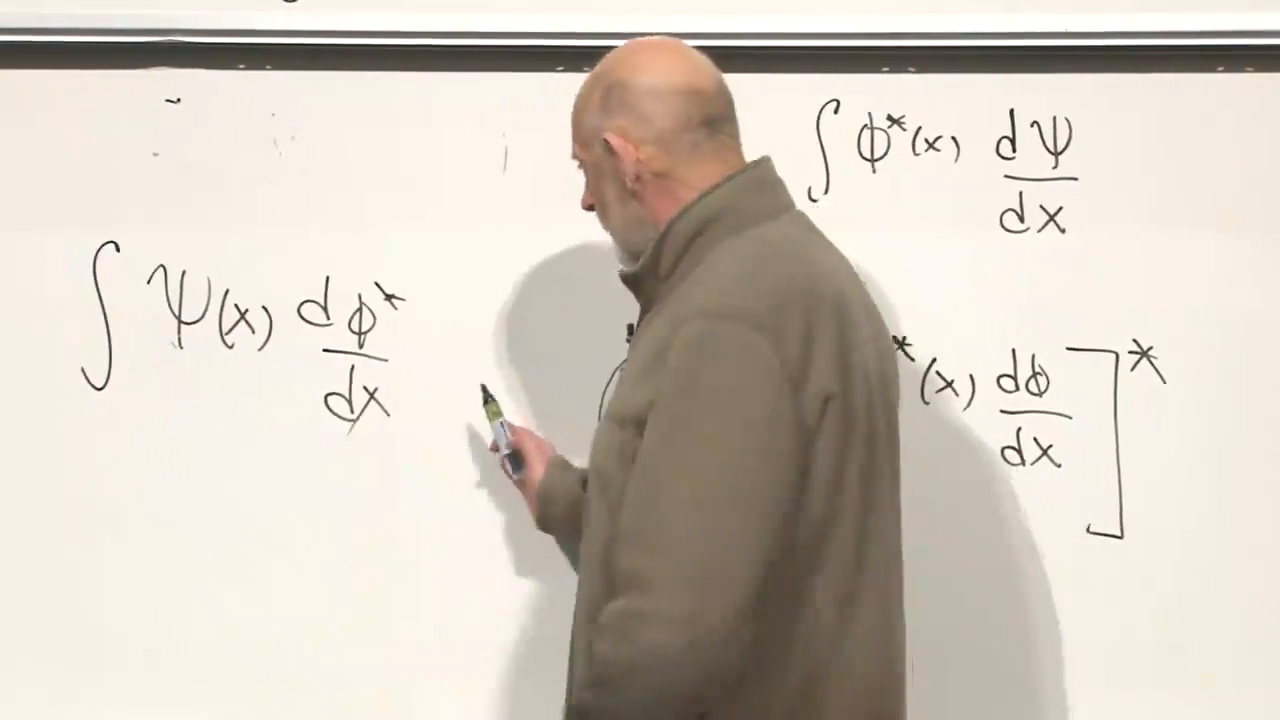
\includegraphics[width=0.88\textwidth]{lecture_08_figure_11.png}
\caption{分部积分把导数在两个波函数之间移动，并引入决定性的负号。}
\lectureframe{01:32:30}
\end{figure}

乘以 \(-i\)：
\begin{equation}
p=-i\frac{d}{dx}.
\label{eq:l8-momentum-natural-units}
\end{equation}
复共轭把 \(-i\) 变为 \(+i\)，而分部积分又贡献一个负号。两个符号相消，所以 \(p^\dagger=p\)。恢复单位后，
\begin{equation}
p=-i\hbar\frac{d}{dx}.
\label{eq:l8-momentum-operator}
\end{equation}

期望值明确显示出它的实性：
\begin{align}
\expect{p}_\psi
&=
-i\int dx\,\psi^*(x)\frac{d\psi}{dx} \notag\\
&=
i\int dx\,\frac{d\psi^*}{dx}\psi(x) \notag\\
&=
\expect{p}_\psi^*.
\label{eq:l8-momentum-expectation-real}
\end{align}
任何等于自身复共轭的数都是实数，正如可观测量的期望值所必须的那样。

\begin{figure}[htbp]
\centering
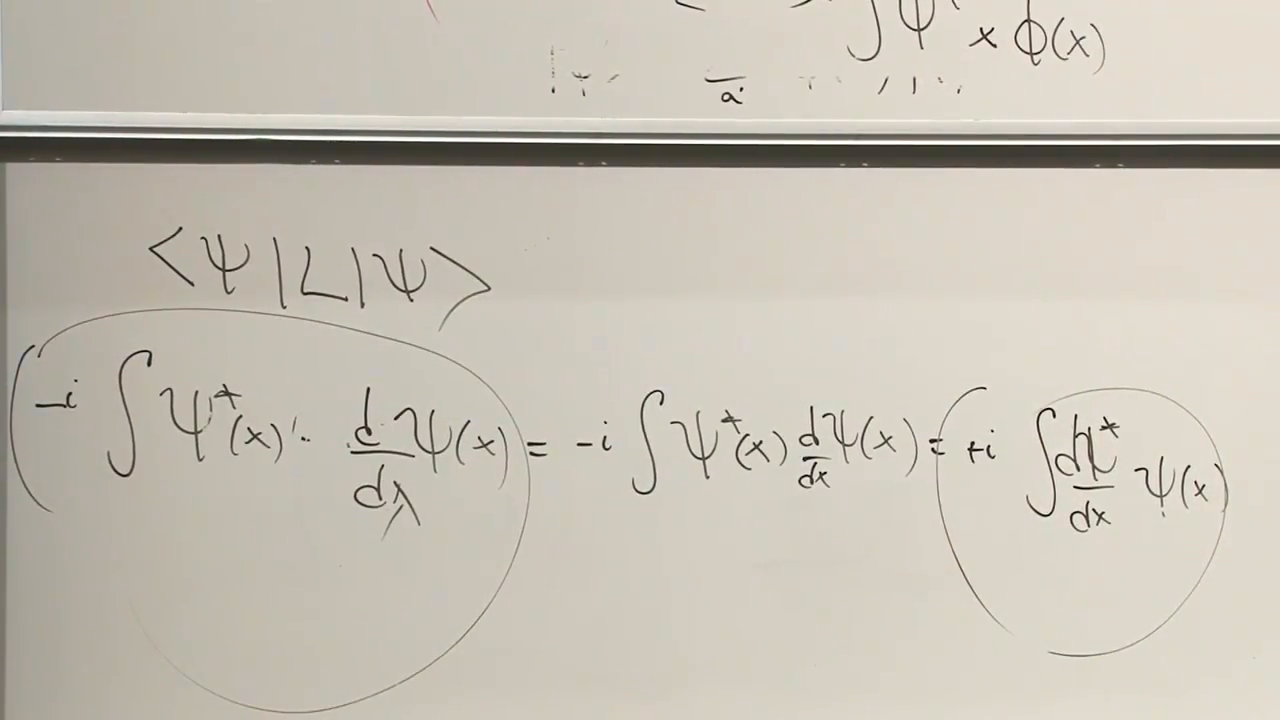
\includegraphics[width=0.88\textwidth]{lecture_08_figure_12.png}
\caption{分部积分前后的动量期望值；这两种形式互为复共轭且相等。}
\lectureframe{01:39:44}
\end{figure}

\begin{classroomqa}
\audiencequestion{为什么一个含有 \(i\) 的算符可以表示实可观测量？}
\lecturerresponse{厄米性涉及的是内积下的整个算符，而不是其坐标公式中的每个符号是否都是实数。因子 \(i\) 补偿了分部积分移动导数时获得的负号，使所有期望值都是实数。}
\end{classroomqa}

\section{正则对易子}

再做一次计算，就能揭示为什么方程~\eqref{eq:l8-momentum-operator}中的算符值得注意。在 \(\hbar=1\) 的单位制下，先用 \(x\) 作用，再用 \(p\) 作用：
\begin{align}
(px\psi)(x)
&=
-i\frac{d}{dx}\bigl(x\psi(x)\bigr) \notag\\
&=
-i\psi(x)-ix\frac{d\psi}{dx}.
\label{eq:l8-px}
\end{align}
交换顺序：
\begin{equation}
(xp\psi)(x)
=
-ix\frac{d\psi}{dx}.
\label{eq:l8-xp}
\end{equation}
从方程~\eqref{eq:l8-xp}中减去方程~\eqref{eq:l8-px}，
\begin{equation}
\bigl([x,p]\psi\bigr)(x)
=
\bigl(xp-px\bigr)\psi(x)
=
i\psi(x).
\end{equation}
因为这对算符定义域中的每个波函数都成立，
\begin{equation}
[x,p]=i,
\end{equation}
或者，恢复单位后，
\begin{equation}
[x,p]=i\hbar.
\label{eq:l8-canonical-commutator}
\end{equation}

\begin{figure}[htbp]
\centering
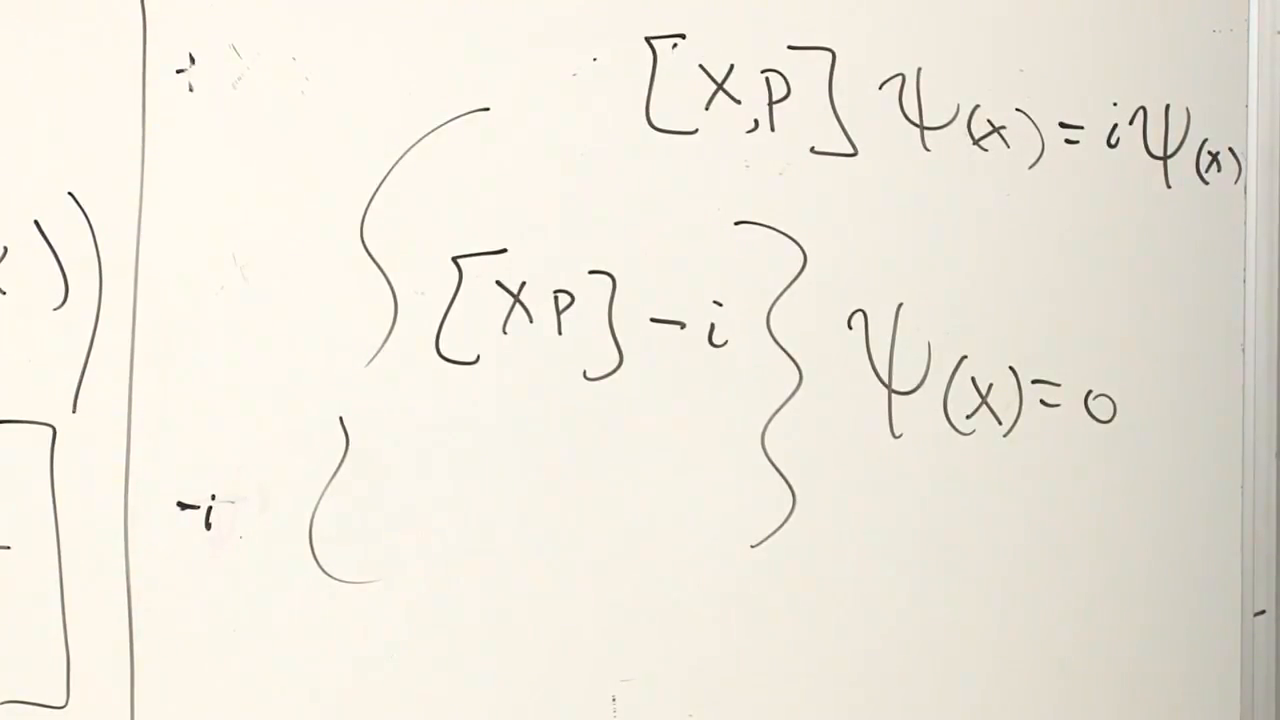
\includegraphics[width=0.88\textwidth]{lecture_08_figure_13.png}
\caption{完成的算符论证：如果对每个波函数都有 \(([x,p]-i)\psi=0\)，那么 \([x,p]=i\)。}
\lectureframe{01:46:24}
\end{figure}

经典对应物是
\begin{equation}
\{x,p\}_{\mathrm{PB}}=1.
\end{equation}
狄拉克的历史性推理方向与当前的推导相反。他从反对称泊松括号与对易子之间的代数相似性出发，假设了对应关系
\begin{equation}
[A,B]\longleftrightarrow i\hbar\{A,B\}_{\mathrm{PB}},
\end{equation}
并推断动量算符必须与位置满足正则对易关系。在这里，我们通过修复导数在厄米性上的失效而发现了\(-i\,d/dx\)，之后才发现同样的代数关系。

\begin{classroomqa}
\audiencequestion{仅凭对易子就能证明\(-i\hbar\,d/dx\)是物理动量吗？}
\lecturerresponse{这是强有力的证据，但并非完整的物理认定。我们仍须证明该算符生成空间平移，在存在平移对称性时其期望值守恒，并且在适当的非相对论系统中波包以群速度\(\expect{p}/m\)运动。}
\end{classroomqa}

\section{接下来是什么}

从自旋到粒子的转变保留了架构，同时改变了其尺度。连续标记的基取代了有限的基矢量列表。求和变为积分，克罗内克{\proseunicodefont δ}变为狄拉克{\proseunicodefont δ}，列矢量变为平方可积函数。位置通过乘法作用，而动量通过微分作用。

接下来的任务与其说是记号上的，不如说是物理上的。动量概率需要动量基和傅里叶变换。时间演化需要关于\(\psi(x,t)\)的Schr\"odinger方程。波包随后将把抽象算符\(p=-i\hbar\,d/dx\)与运动联系起来：其群速度将与动量除以质量相关，而平移对称性将解释动量守恒。因此，对易关系\([x,p]=i\hbar\)并非孤立的技巧。它是已经建立的矢量空间力学与粒子量子动力学之间的枢纽。
